Inductive learning of symbolic expression for continuous-valued time series
data is a hard task which has recently been tackled using a greedy search over 
the approximate posterior of the possible kernel compostions for
\ac{GP}s~\citep{duvenaud2013structure,lloyd2014automatic}\footnote{\url{http://www.automaticstatistician.com/}}.

With \gpmem\ we can provide a fully Bayesian treatment of this, previously unavaible,
using a stochastic grammar  (see Fig. \ref{fig:schema}).

\begin{figure}
\centering
\usetikzlibrary{arrows, decorations.markings}
\usetikzlibrary{trees}

\tikzstyle{level 1}=[level distance=1cm, sibling distance=1.5cm]
\tikzstyle{level 2}=[level distance=1cm, sibling distance=1.1cm]

% Define styles for operators and leafs
\tikzstyle{operator} = [draw=none,circle, minimum width=1pt]
\tikzstyle{end} = [circle, minimum width=3pt,fill, inner sep=0pt]
% for double arrows a la chef
% adapt line thickness and line width, if needed

\begin{subfigure}[b]{0.49\textwidth}\centering
\begin{tikzpicture}[thick]
 \node[] (start) {};
 \node[left=-0.2cm of start] (base_kernels) {\small$\{\Kbf_{\bm{\theta}^1}^1,\cdots,\Kbf_{\bm{\theta}^m}^m\}$};
 \node[above=0.7cm of base_kernels] (theta) {\small$\bm{\theta}^* \sim P(\bm{\theta}^*)$};
\node[right=0.5cm of start] (n) {$P(n)$};
 \node[draw,rectangle, below=1cm of start, text width =6.0cm, text 
height=4.1cm,align=center] (grammar)
{};


 \node[draw,dashed,rectangle, below=-3.8cm of grammar, text width
=4.7cm,align=center] (subset) {
$\;\;\;\;\;\;\;\;\;\;\;\;$Subset SP % I can't believe that this is the simpliest way to
% get spacing right 
{\raggedright
\footnotesize$ n\; \sim P(n),\;\;\;\;\; n \leq m$ \\

\footnotesize$S \; \sim P(S = \{\Kbf_{\bm{\theta}^i}^i,\cdots,\Kbf_{\bm{\theta}^n}^n\} \mid n)$
}
};
 \node[draw,rectangle,dashed, below=0.7cm of subset, text width
=4.35cm,align=center]
(composition_procedure) {
$\;$Composition Procedure\\ % I can't believe that this is the simpliest way to
% get spacing right 
{\raggedright
\footnotesize$\bm{\Omega}\;\; \sim P(\bm{\Omega} \mid S,n)$ \\

\footnotesize$\Kbf_{\bm{\theta}} \sim P(\Kbf_{\bm{\theta}} \mid \bm{\Omega},S,n),\;\,\bm{\theta}\subseteq\bm{\theta}^*$
}
};

\node[above=0.0cm of subset]{\centering \bf Stochastic Grammar}; 

 \node[draw,rectangle,below=1cm of grammar] (gpmem) {\texttt{gpmem}};

 \node[draw,rectangle,below=1cm of gpmem] (f) {Data Generation};
\node[left of=f,xshift=-1.5cm] (x) {$\mathbf{t}$};
\node[right of=f,xshift=1.5cm] (y) {$\mathbf{f}$};

 \node[below=0.1cm  of grammar,xshift=0.5cm] (k)
{\small$\Kbf_{\bm{\theta}}$};


\node[below=0.1cm  of gpmem,xshift=0.6cm] (gp) {
\small$f_{emu}$};

% 1st pass: draw arrows
  \draw[thick,->] (base_kernels) -- (grammar);
  \draw[thick,->] (n) -- (grammar);
  \draw[thick,->] (theta) -- (base_kernels);
  \draw[thick,->] (grammar) -- (gpmem);
  \draw[thick,->] (gpmem) -- (f);
 \draw[thick,->] (x) -- (f);
 \draw[thick,->] (f) -- (y);
 \draw[thick,dashed,->] (subset) -- node[right]{\footnotesize $\;S$} (composition_procedure);
  % Note: If you have no branches, the 2nd pass is not needed
\end{tikzpicture}\vspace{2mm}
\caption{} 
\end{subfigure}
\begin{subfigure}[b]{0.49\textwidth}\centering
\begin{tikzpicture}[grow=right, sloped]
\node[operator] {\small $+$}
    child {
        node[operator] {\small $+$}        
            child {
               node[operator] {\small $\times$}        
        child {
                node[operator, label=right:
                    {$\cdots$}] {}
                edge from parent
                node[above] {}
                node[below]  {}
            }
            child {
                node[end, label=right:
                    {SE$_{\theta^4}$}] {}
                edge from parent
                node[above] {}
                node[below]  {}
            }
        edge from parent         
            node[above] {}
            node[below]  {}
            }
            child {
                node[end, label=right:
                    {WN$_{\theta^3}$}] {}
                edge from parent
                node[above] {}
                node[below]  {}
            }
            edge from parent 
            node[above] {}
            node[below]  {}
    }
    child {
        node[operator] {\small $\times$}        
        child {
                node[end, label=right:
                    {PER$_{\theta^2}$}] {}
                edge from parent
                node[above] {}
                node[below]  {}
            }
            child {
                node[end, label=right:
                    {LIN$_{\theta^1}$}] {}
                edge from parent
                node[above] {}
                node[below]  {}
            }
        edge from parent         
            node[above] {}
            node[below]  {}
    };
\node[xshift=-0.7cm] (K) {$\mathbf{K}_{\bm{\theta}}=$}; 
 \node[xshift=2.6cm,below =2.4cm of K] (Keq) {$\mathbf{K}_{\bm{\theta}}=\text{LIN}_{\theta^1} \times \text{PER}_{\theta^2}+\text{WN}_{\theta^3} + \text{SE}_{\theta^4} \times ( \cdots )$};
\end{tikzpicture}
\caption{} 
\end{subfigure}

\begin{subfigure}[b]{0.99\textwidth}\centering
\begin{tabular}{cccc}
\multicolumn{4}{c}{\bf Base Components} \rule{0pt}{3ex} \\ 
\small LIN: Linearity &\small PER: Periodicity &\small SE: Smoothness &\small WN: White Noise \rule{0pt}{2ex} \\
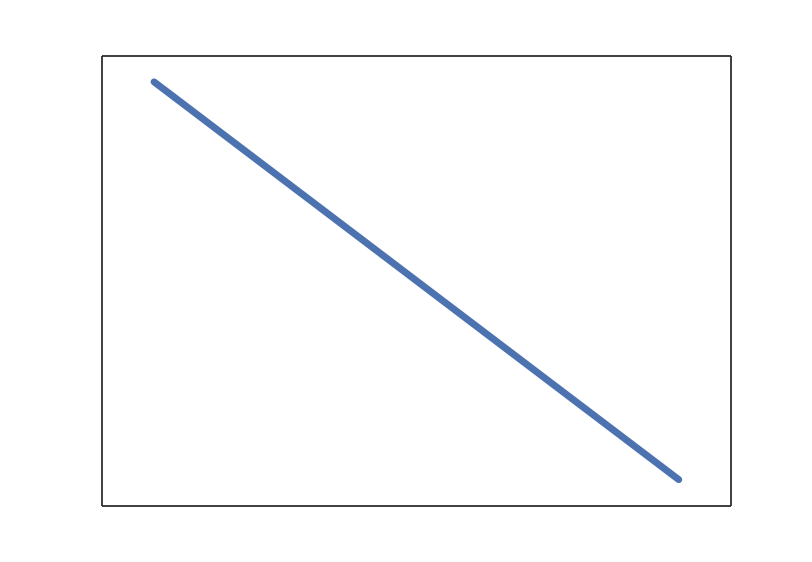
\includegraphics[height=2cm]{figs/kernel/kernelLIN.png} & 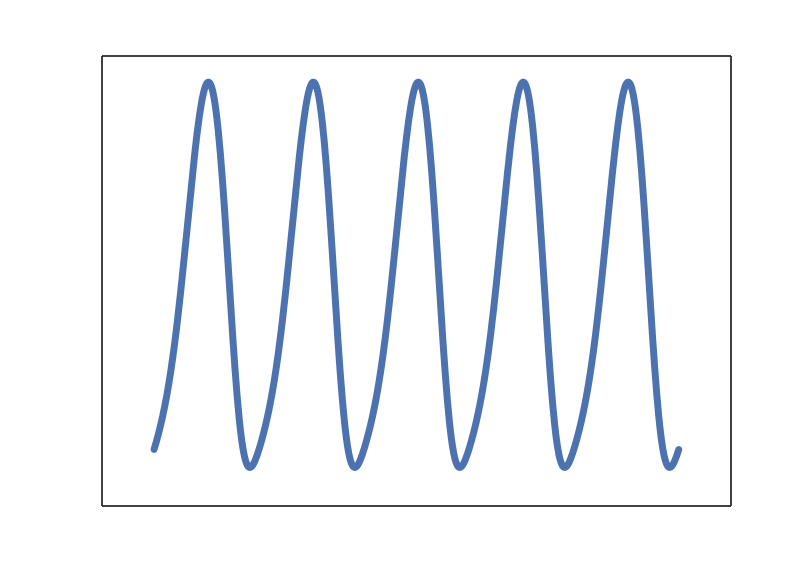
\includegraphics[height=2cm]{figs/kernel/kernelPER.png} & 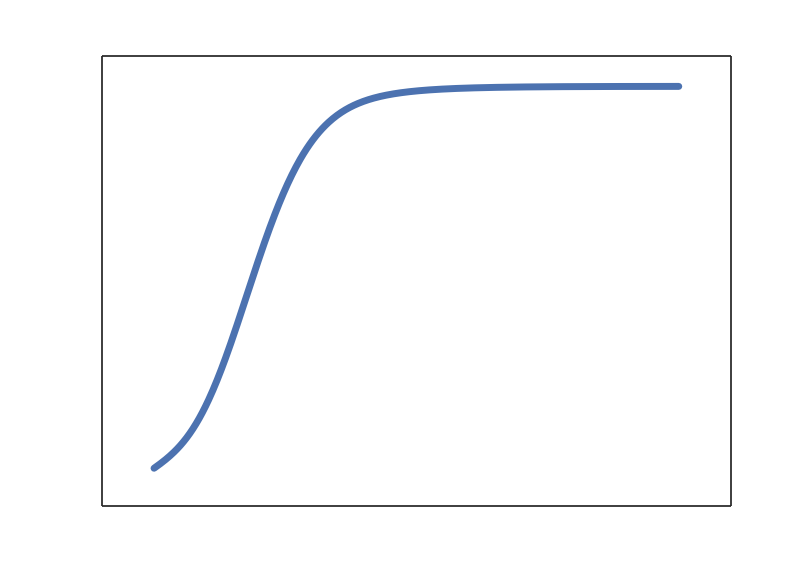
\includegraphics[height=2cm]{figs/kernel/kernelSE.png} & 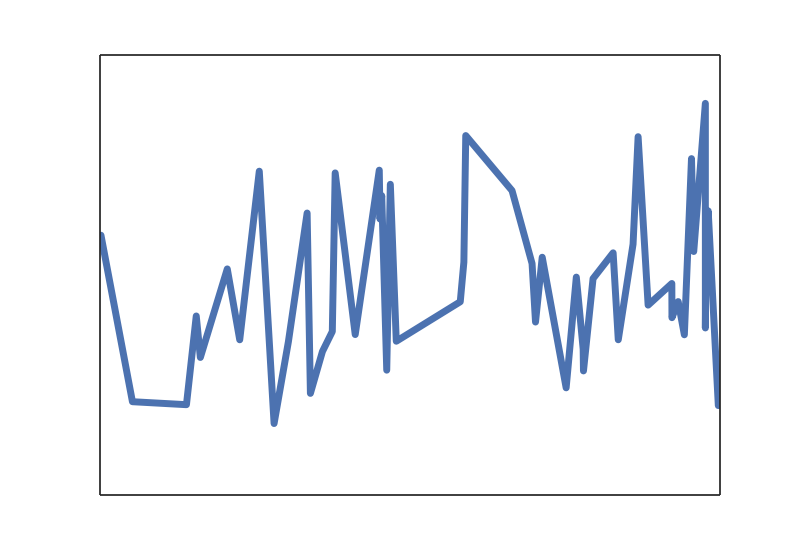
\includegraphics[height=2cm]{figs/kernel/kernelWN.png}\\
\end{tabular}
\begin{tabular}{cccc}
\multicolumn{4}{c}{\bf Composite Structure} \rule{0pt}{0ex}  \\ 
\small LIN + PER: &\small LIN $\times$ PER: &\small SE $\times$ PER: &\small LIN $\times$ LIN: \rule{0pt}{2ex} \\
\small Periodicity with Trend &\small Growing Amplitude &\small Local Periodicity&\small Quadratic \rule{0pt}{2ex} \\
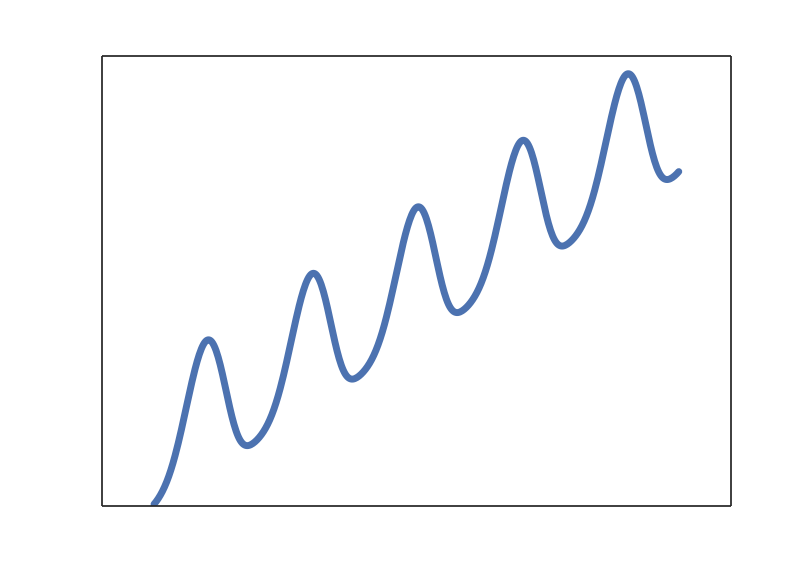
\includegraphics[height=2cm]{figs/kernel/kernelLINplusPER.png} & 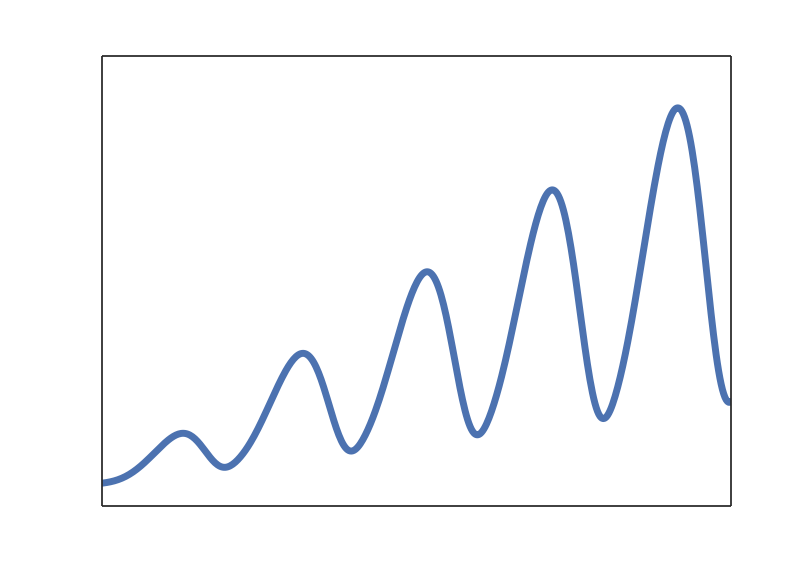
\includegraphics[height=2cm]{figs/kernel/kernelLINtimesPER.png} & 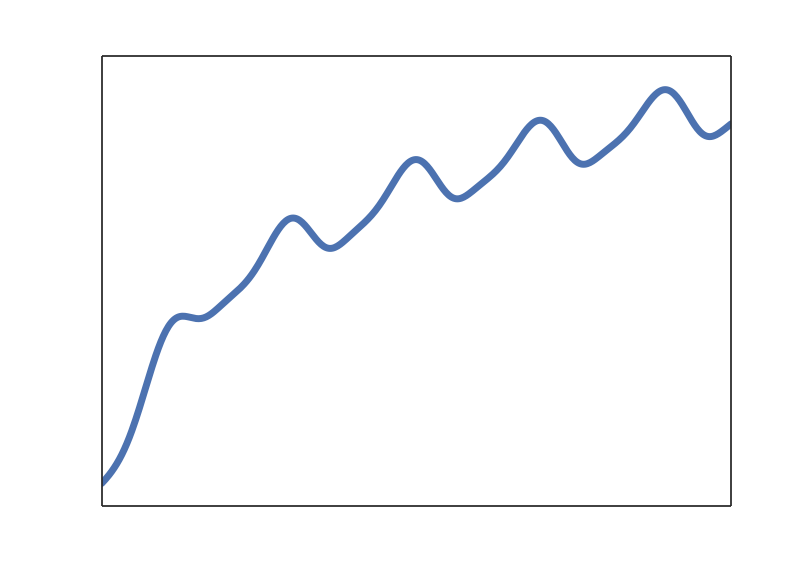
\includegraphics[height=2cm]{figs/kernel/kernelSEplusPER.png}& 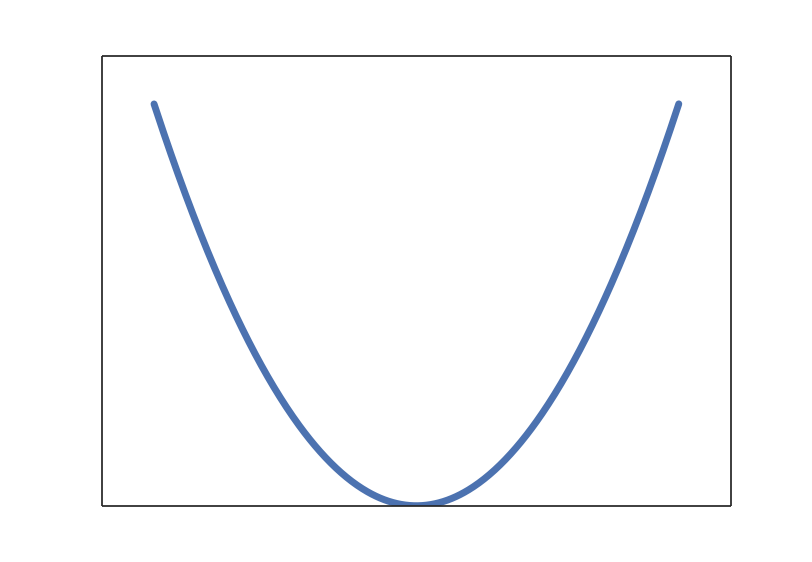
\includegraphics[height=2cm]{figs/kernel/kernelLINtimesLIN.png}\\
\end{tabular}
\caption{}
\end{subfigure}

\caption{(a) Graphical description of Bayesian GP structure learning. (b) Composite structure. (c) The natural language interpretation of the structure.}\label{fig:schema}
\end{figure}

We deploy a probabilistic context free grammar for our prior on structures. An input of non-composite kernels (base kernels) is supplied to generate a posterior distributions of composite structure to express local and global aspects of the data.


We approximate the following intractable integrals of the expectation for the prediction:
\begin{equation}
\mathbb{E}[y^* \mid x^*,\mathbf{D},\mathbf{K}] =\iint f(x^*,\bm{\theta},\mathbf{K})\,P(\bm{\theta} \mid \mathbf{D,\mathbf{K}})\,P(\mathbf{K}|\bm{\Omega},s,n) \; \mathbf{d} \bm{\theta} \mathbf{d} \mathbf{K}.  
\end{equation}

This is done by sampling from the posterior probability distribution of the hyper-parameters and the possible kernel:
\begin{equation}
y^* \approx \frac{1}{T} \sum^T_{t=1} f(x^* | \bm{\theta}^{(t)},\mathbf{K}^{(t)}). 
\end{equation}


In order to provide the sampling of the kernel, we introduce a stochastic process that simulates the grammar for algebraic expressions of covariance function algebra:
\begin{equation}
\mathbf{K}^{(t)} \sim  P(\mathbf{K} \mid \bm{\Omega},s,n)
\end{equation}
Here, we start with the set of given base kernels and draw a random subset.
For this subset of size $n$, we sample a set of possible operators $\bm{\Omega}$ combining base kernels. 
The marginal probability of a composite structure
\begin{equation}
P(\mathbf{K} \mid \bm{\Omega},s,n) = P(\bm{\Omega} \mid s,n)\times P(s \mid n) \times P(n),
\end{equation}
is characterized by the prior $P(n)$ on the number of base kernels used, the probability of a uniformly chosen subset of the set of $n$ possible covariance functions
\begin{equation}
\label{eq:subsets}
P(s \mid n) = \frac{n!}{ \mid s \mid !},
\end{equation}
and the probability of sampling a global or a local structure, which is given by a binomial distribution: 
\begin{equation}
P(\bm{\Omega} \mid s,n)= {n \choose r}  p_{+\times}^k (1 - p_{+\times})^{n-k}.
\end{equation}



Many equivalent covariance structures can be sampled due to covariance function algebra and equivalent representations with different parameterization~\citep{lloyd2014automatic}. To inspect the posterior of these equivalent structures we convert each kernel expression into a sum of products and subsequently simplify. All base kernels can be found in Appendix A, rules for this simplification can be found in appendix B. The code for learning of kernel structure is as follows:

\begin{mdframed}
\begin{minipage}{\linewidth}
\small
\belowcaptionskip=-10pt
\begin{lstlisting}[mathescape,label=alg:structureVent,basicstyle=\selectfont\ttfamily,numbers=none,escapechar=\#]
// GRAMMAR FOR KERNEL STRUCTURE
#\linenumber{1}#assume kernels = list(se, wn, lin, per, rq) // defined as above

// prior on the number of kernels
#\linenumber{2}#assume p_number_k = uniform_structure(n)
#\linenumber{3}#assume subset_kernels = tag(quote(grammar), 0,
#\linenumber{4}#                            subset(kernels, p_number_k))

// kernel composition
#\linenumber{5}#assume composition = proc(l) {
#\linenumber{6}#  if (size(l) <= 1) {
#\linenumber{7}#    first(l)
#\linenumber{8}#  } else {
#\linenumber{9}#    if (bernoulli()) {
#\linenumber{10}#      add_funcs(first(l), composition(rest(l)))
#\linenumber{11}#    } else {
#\linenumber{12}#       mult_funcs(first(l), composition(rest(l)))
#\linenumber{13}#    }
#\linenumber{14}#  }
#\linenumber{15}#}

#\linenumber{16}#assume K = tag(quote(grammar), 1, composition(subset_kernels))

// APPLY GPMEM
#\linenumber{17}#assume (f_compute, f_emu) = gpmem(f_look_up, K)

// Probe all data points
#\linenumber{18}#for n ... N
#\linenumber{19}#  predict f_compute(get_data_xs(n))

// PERFORMING INFERENCE
#\linenumber{20}#infer repeat(200, do(
#\linenumber{21}#  mh(quote(grammar), one, 1),
#\linenumber{22}#  for kernel in K:
#\linenumber{23}#    mh(quote(parameters$_{\text{kernel}}$), one, 1)))
\end{lstlisting}

\end{minipage}
\end{mdframed}


We defined the space of covariance structures in a way that allows us to produce results coherent with 
work presented in Automatic Statistician. For example, for the airline data set describing monthly totals of international airline passengers (\citealp{box2011time}, according to \citealp{duvenaud2013structure}). Our most frequent sample is identical with the highest scoring result reported in previous work using a search-and-score method~\citep{duvenaud2013structure} for the CO$_2$ data set (see \citealp{rasmussen2006gaussian} for a description) and the predictive capability is comparable. However, the components factor in a different way due to different parameterization of the individual base kernels. We see that the most probable alternatives for a structural description both recover the data dynamics (Fig. \ref{fig:posterior_twosamples} for the airline data set).

Confident about our results, we can now query the data for certain structures being present. We illustrate this using the Mauna Loa data used in previous work on automated kernel discovery~\citep{duvenaud2013structure}. We assume a relatively simple hypothesis space  consisting of only four kernels, a linear, a smoothing, a periodic and a white noise kernel. In this experiment, we resort to the white noise kernel instead RQ (similar to \citep{lloyd2014automatic}).  We can now run the algorithm, compute a posterior of structures (see Fig. \ref{fig:posterior}). We can also query this posterior distribution for the marginal of certain simple structures to occur. We demonstrate this in Fig. \ref{fig:query}
\begin{figure}
\centering
 \addtolength\abovedisplayskip{-1\baselineskip}%
  \addtolength\belowdisplayskip{-1\baselineskip}%
 
\begin{tikzpicture}
\node (datatitle) {\small Raw Data};
\node[below = -0.25cm of datatitle] (data) {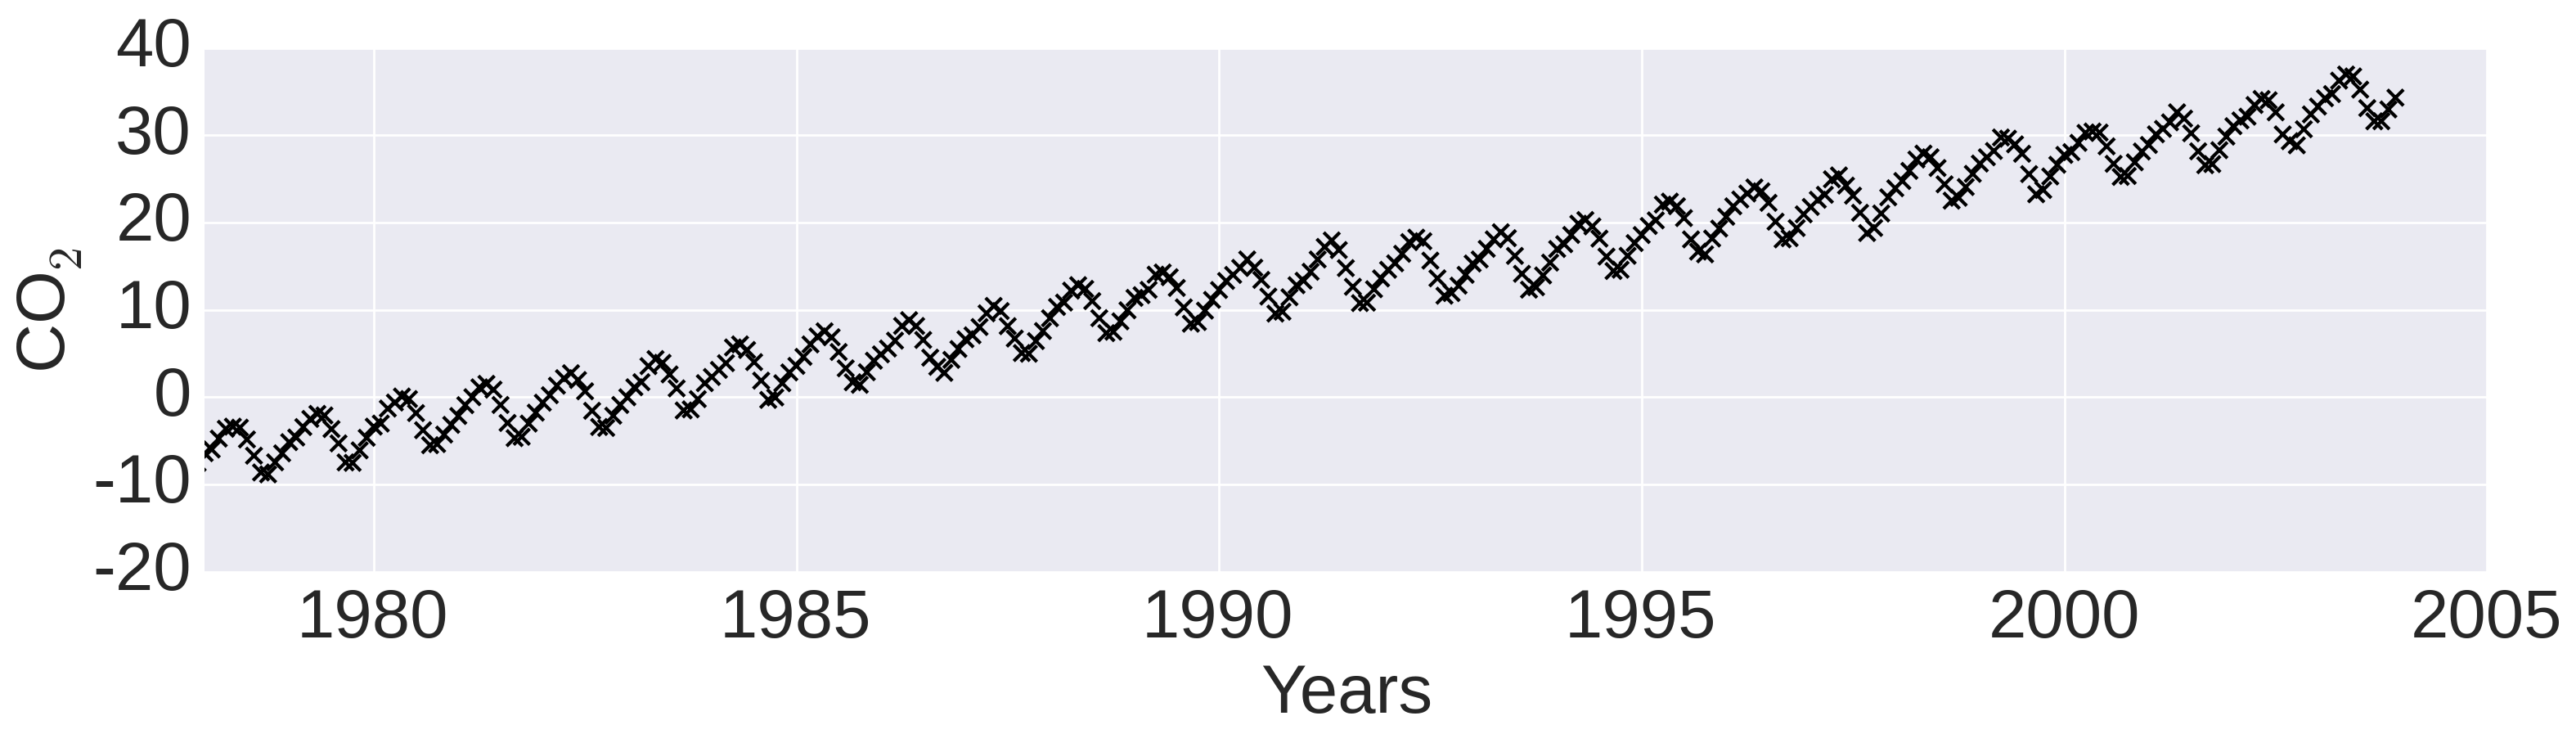
\includegraphics[width=0.7\textwidth]{figs/mauna_data.png}};
\node[below = 2.5cm of data] (post_param_helper) {};
\node[above = 1cm of post_param_helper] (post_param_helper_1) {};
\node[below = 1cm of post_param_helper] (post_param_helper_2) {};
\node[left = -3cm of post_param_helper] (post_param) {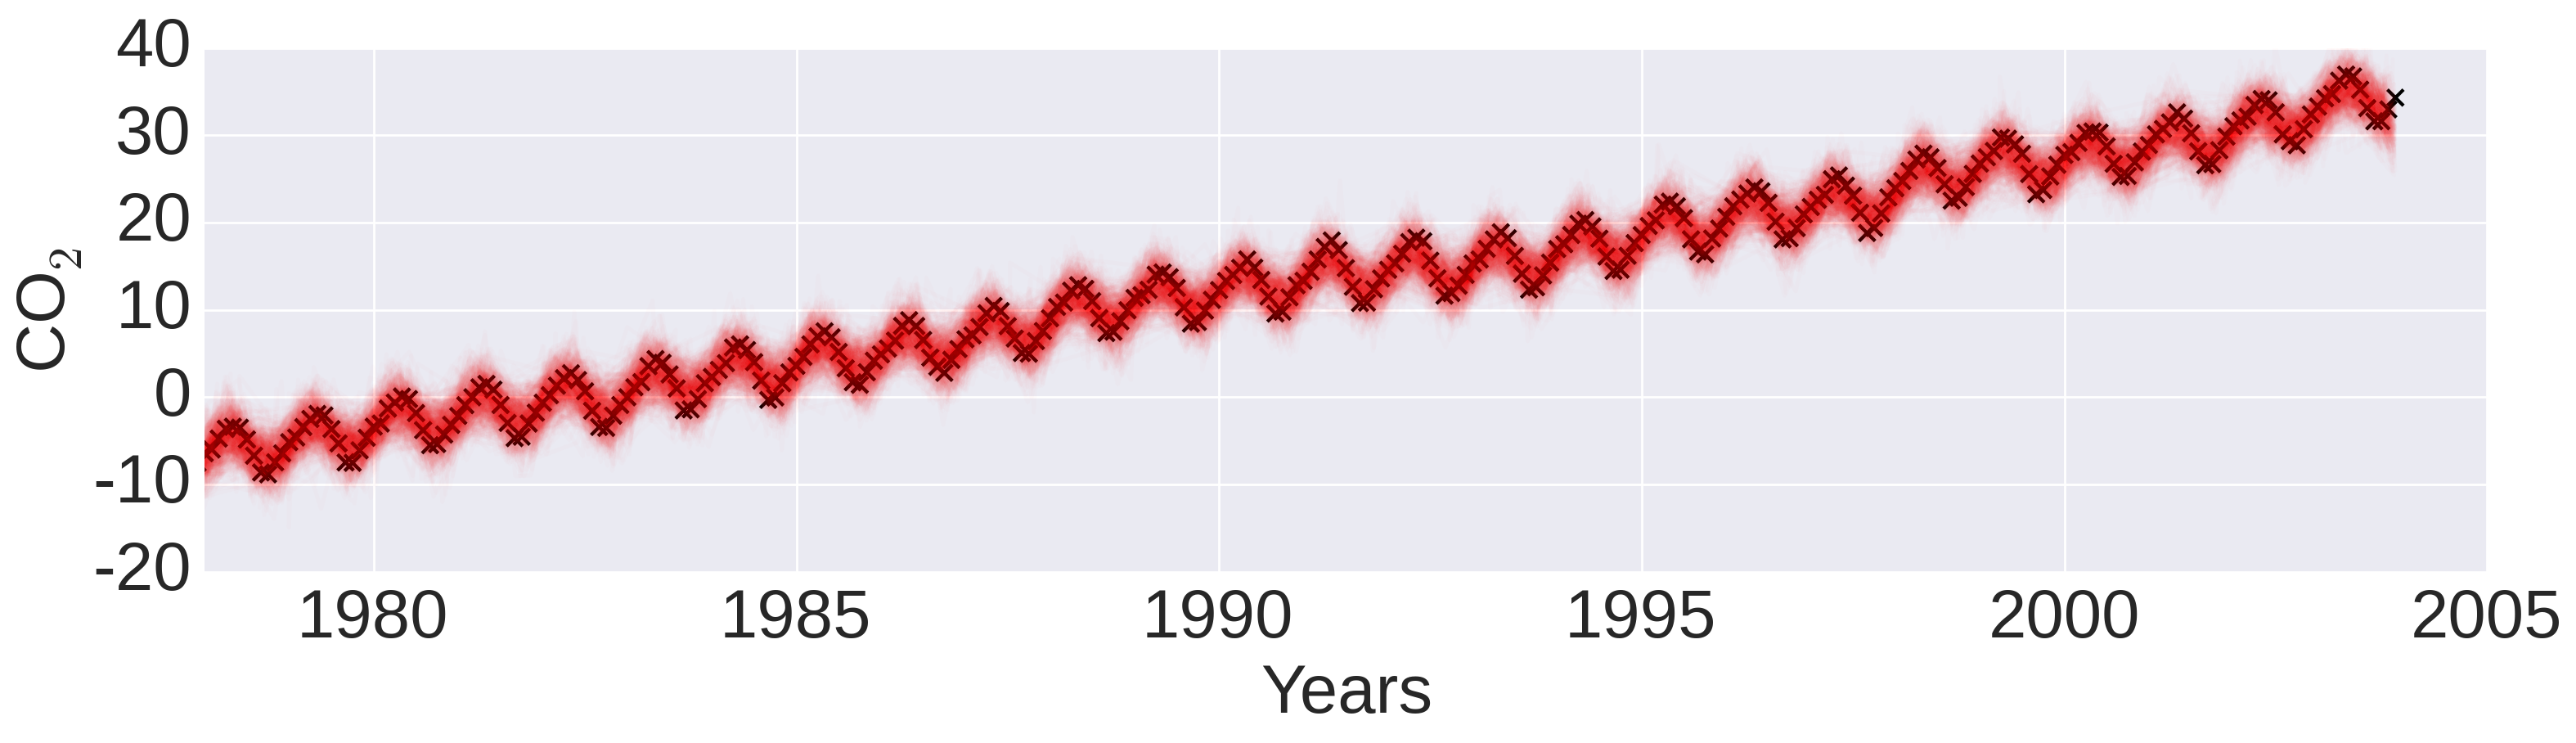
\includegraphics[width=0.6\textwidth]{figs/mauna_sample_1.png}};
\node[draw,rectangle,color=red,dashed,right = 4.5cm of post_param_helper,yshift=0.3cm] (zoom) {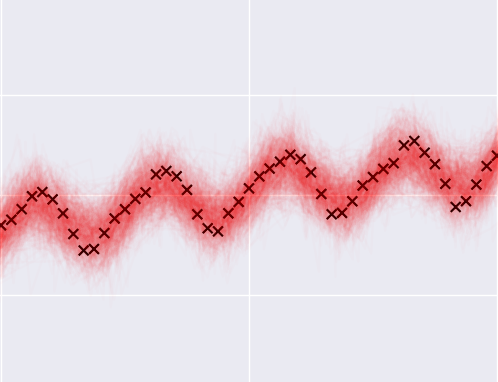
\includegraphics[width=0.2\textwidth]{figs/mauna_zoom.png}};
\node[draw,rectangle,color=red,dashed,left = 3.8cm of zoom, minimum width =
1.5cm, minimum height = 1.2cm,yshift=0.0cm] (zoom_in) {};
\node[below = 1.2cm of post_param_helper_2] (posterior) {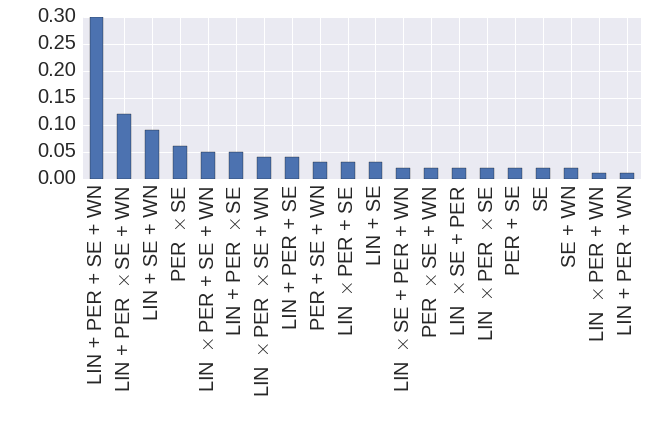
\includegraphics[width=0.6\textwidth]{figs/mauna_structure.png}};

\node[draw,rectangle,below = 1.2cm of posterior] (formula_param_1) {\color{black}\small
$\Ktheta= 2.7^2(x x^\prime) + 5.6^2 \exp \bigg( \frac{2 \sin^2 ( \pi (x - x^\prime)/3.7}{6.4^2} \bigg)
+ 0.4^2 \exp(-\frac{(x-x^\prime)^2}{2 \times 6.3^2}) +  1.9^2 \delta_{x,x^\prime} \label{eq:WN}$ };


\node[draw,rectangle,below = 1.2cm of formula_param_1,text width =
0.9\textwidth,minimum height = 1.5cm,font=\footnotesize] (paragraph){
The posterior peaks at a kernel structure with four additive components. Additive components hold globally, that is there are no higher level, qualitative aspects of the data that vary with the input space. The additive components are as follows: (i) a linearly increasing function or trend; (ii) a periodic function; (iii) a smooth function; and (iv) white noise.};







\node[draw, rectangle, left = -1.75cm of posterior,minimum width = 0.45cm, minimum height = 5.8cm,yshift=0.2cm] (mark_structure) {};
%\node[draw,very thick, rectangle, below = 1.1cm of data,minimum width = \textwidth, minimum height = 15cm] (posterior_frame) {};

%\node[left = 1.3cm of mark_structure] (paragraph_helper){};
\node[below =0.45cm of mark_structure,inner sep = 0pt,outer sep=0pt] (formula_helper) {};
\node[above =1.2cm of formula_param_1,inner sep = 0pt,outer sep=0pt] (formula_helper_2) {};

%\draw[-,dashed] (mark_structure.south) -- (formula_helper);
%\draw[-,dashed] (formula_helper) -- (formula_helper_2);
%\draw[->,dashed] (mark_structure) -- (paragraph_helper);
%\draw[->,dashed] (formula_helper_2) -- (formula);

\draw[->] (data) -- node[right]{\small $\hat \fbf \sim
\mathcal{N}(\hat{\bm{\mu}},\hat\Kbf)$} (post_param_helper_1);
\draw[->] (post_param_helper_2) -- node[right]{\small Posterior Structure} (posterior);
\draw[->] (formula_helper_2) -- node[right] {\small
$\bm{\theta}=\{2.7,5.6,3.7,6.4,0.4,6.3,1.9\}$} (formula_param_1);
\draw[-] (mark_structure) -- node[left, yshift=-0.3cm] {\small $\Ktheta$} (formula_helper);
\draw[-] (formula_helper) --(formula_helper_2);
\draw[->] (formula_param_1) -- node[right]{\small Qualitative Interpretation} (paragraph);

\draw[->,dashed,red] (zoom_in) --node[above]{\small\color{red}Zoom in:}
node[below]{\small\color{red}adequate error bars}(zoom);

%\draw[->,line width=1pt,double distance=2pt] (data) -- (post_param);
% starting from the bottom to aligm with caption 
\node[left=0.3cm of paragraph] (e){(e)}; 

\node[above=1.9cm of e] (d) {(d)}; 
\node[above=5.0cm of d] (c) {(c)}; 
\node[above=4.7cm of c] (b) {(b)}; 
\node[above=4.0cm of b] (a) {(a)}; 
\end{tikzpicture}
\addtolength\abovedisplayskip{1\baselineskip}%
\addtolength\belowdisplayskip{1\baselineskip}%



\caption{Posterior of structure and qualitative, human interpretable reading. We take the raw data (top), compute a posterior distribution on structures (red samples and bar plot).
We take the peak of this distribution ($\text{LIN}+\text{PER}+\text{SE}+\text{WN}$) with the sampled parameters used to generate the samples for the second plot from the top. We  its human readable interpretation (left of bar plot).}\label{fig:posterior}
\end{figure}

\begin{figure}
\centering
 \addtolength\abovedisplayskip{-1\baselineskip}%
  \addtolength\belowdisplayskip{-1\baselineskip}%
  
\begin{tikzpicture}
\node (datatitle) {\small Raw Data};
\node[below = -0.25cm of datatitle](data) {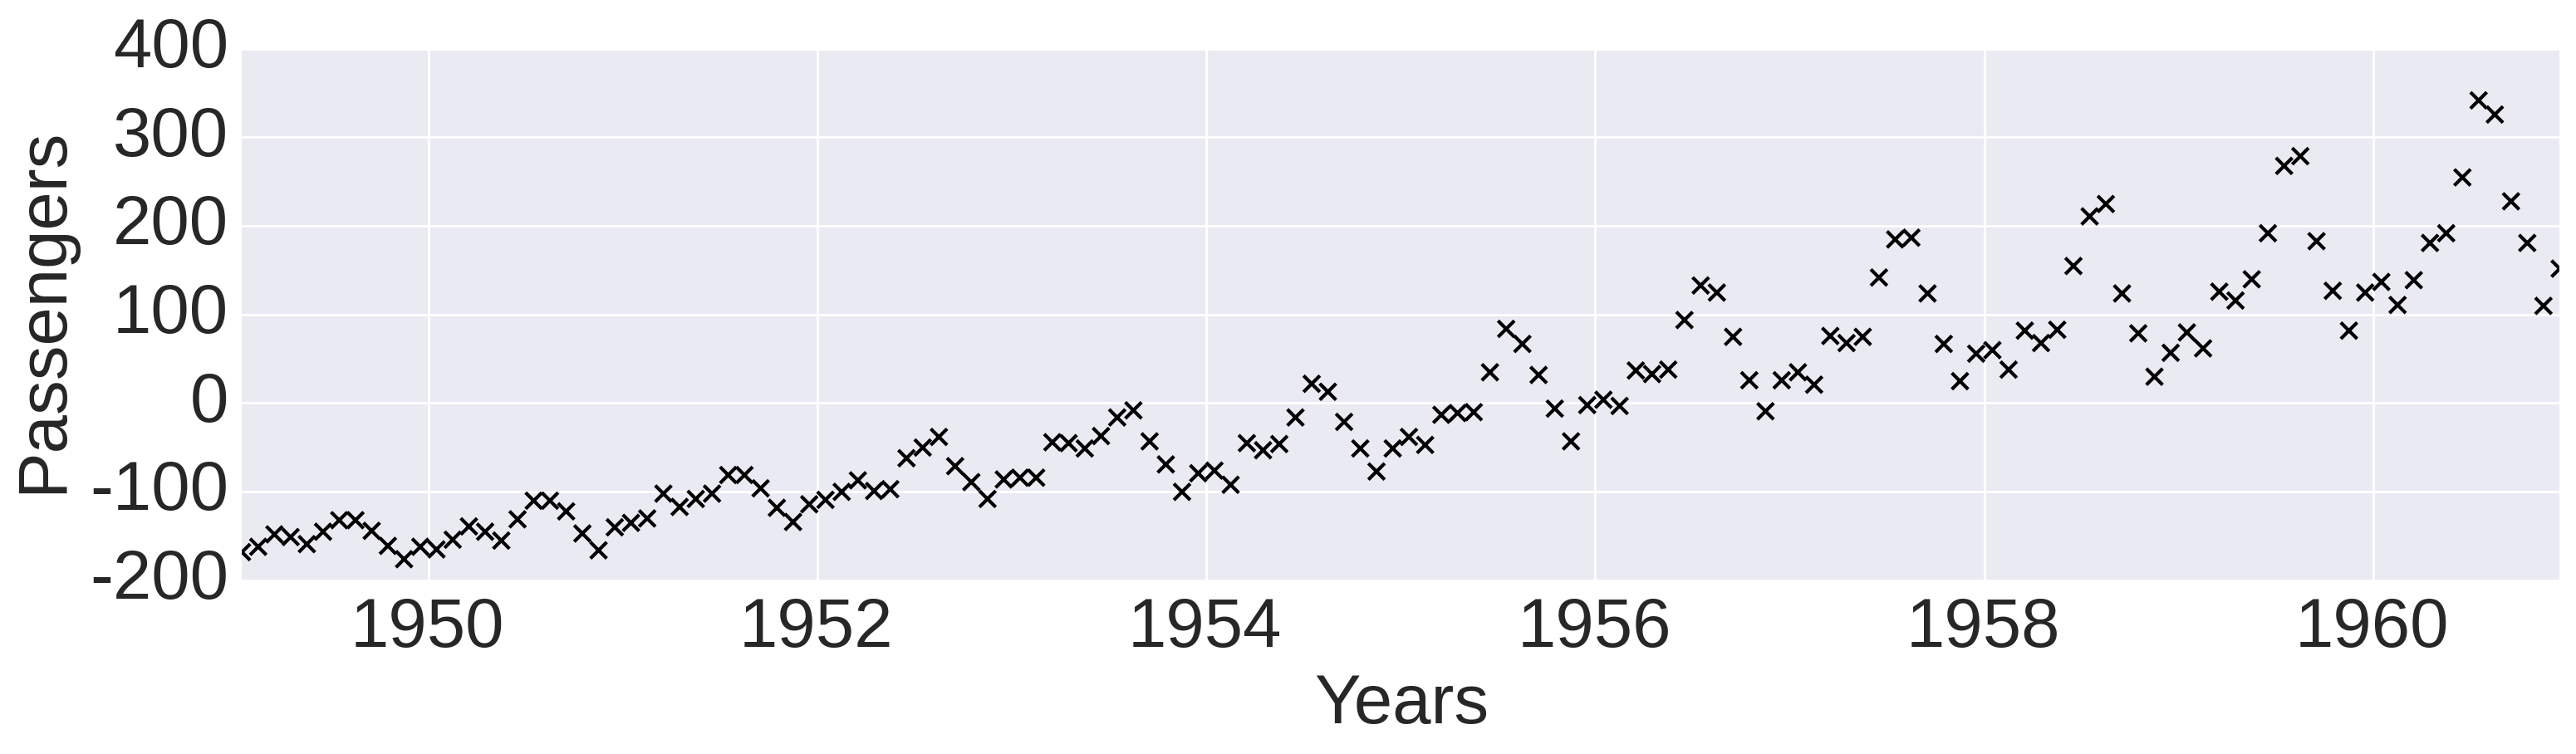
\includegraphics[width=0.65\textwidth]{figs/airline_data.png}};
\node[below= 1.2cm of data] (post_param) {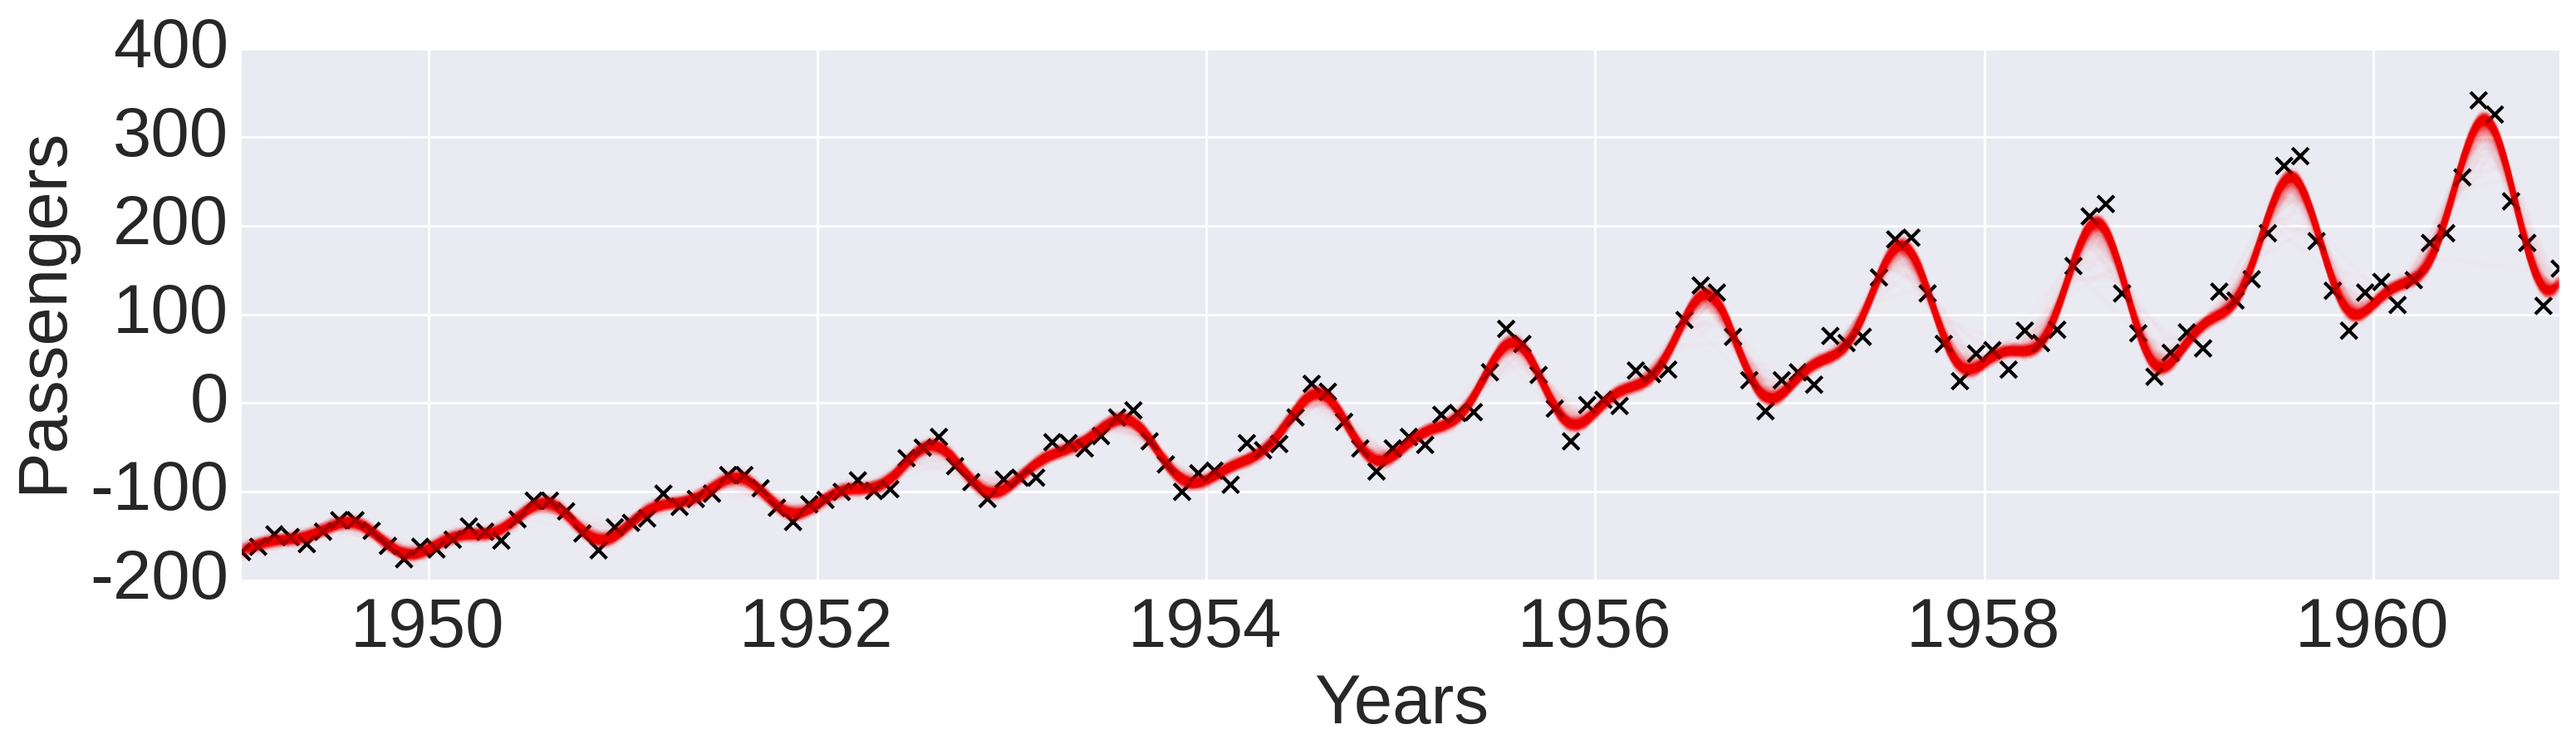
\includegraphics[width=0.65\textwidth]{figs/airline_sample_28.png}};


\node[below = 1.2cm of post_param] (posterior) {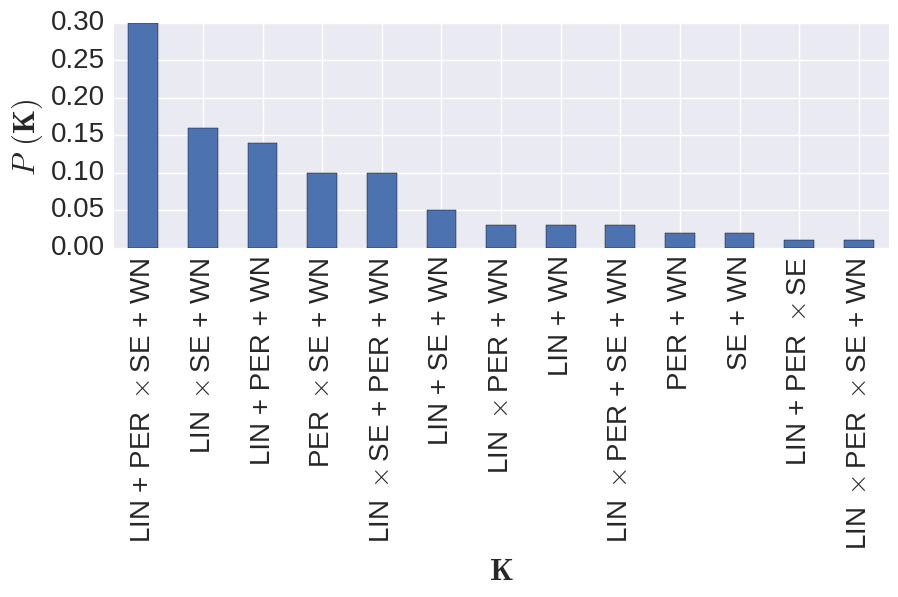
\includegraphics[width=0.55\textwidth]{figs/airline_structure.png}};
\node[below=-0.7cm of posterior,xshift=0.3cm] (xlabel) {\footnotesize
$\Ksrv$};
\node[left =-0.5cm of posterior,yshift=1.3cm] (ylabel) {\rotatebox{90}{\footnotesize
$P(\Ksrv \mid \xbf,\ybf, \thetabf )$}};
\node[draw,rectangle,below = 1.2cm of posterior] (formula_param_1) {\small\color{black}
$\ktheta= 7.47^2(x x^\prime) +
\Bigg(0.27^2 \exp(-\frac{(x-x^\prime)^2}{2 \times 4.63^2}) \times 
7.34^2 \exp \bigg( \frac{2 \sin^2 ( \pi (x - x^\prime)/4.4}{4.55^2} \bigg)\Bigg)
+ 2.93^2 \delta_{x,x^\prime} \label{eq:WN}$ };


\node[draw,rectangle,below = 1.2cm of formula_param_1,text width =0.9\textwidth,minimum height = 1.5cm, font=\footnotesize] (paragraph){ 
The posterior peaks at a kernel structure with three additive components.
Additive components hold globally, that is there are no higher level,
qualitative aspects of the data that vary with the input space. The additive
components are as follows: (i) a linearly increasing function or trend; (ii) an approximate periodic function; and (iv) white noise.};







\node[draw, rectangle, left = -1.7cm of posterior,minimum width = 0.45cm, minimum height = 5.2cm,yshift=0.2cm] (mark_structure) {};
%\node[draw,very thick, rectangle, below = 1.1cm of data,minimum width = \textwidth, minimum height = 15cm] (posterior_frame) {};

%\node[left = 1.3cm of mark_structure] (paragraph_helper){};
\node[below =0.45cm of mark_structure,inner sep = 0pt,outer sep=0pt] (formula_helper) {};
\node[above =1.2cm of formula_param_1,inner sep = 0pt,outer sep=0pt] (formula_helper_2) {};

%\draw[-,dashed] (mark_structure.south) -- (formula_helper);
%\draw[-,dashed] (formula_helper) -- (formula_helper_2);
%\draw[->,dashed] (mark_structure) -- (paragraph_helper);
%\draw[->,dashed] (formula_helper_2) -- (formula);

\draw[->] (data) -- node[right]{\small $\yprime \sim
\mathcal{N}(\mupost,\Kpost)$} (post_param_helper_1);
\draw[->] (post_param_helper_2) -- node[left]{\small }node[right]{\small Marginal on
Structure: $P(\Ksrv \mid \xbf,\ybf,\thetabf )$} (posterior);
\draw[->] (formula_helper_2) -- node[right] {\small
$\bm{\theta}=\{7.47,0.27,4.63,7.34,4.4,4.55,2.93\}$} (formula_param_1);
\draw[-] (mark_structure) -- node[left, yshift=-0.3cm] {\small $\ktheta$} (formula_helper);
\draw[-] (formula_helper) --(formula_helper_2);
\draw[->] (formula_param_1) -- node[right]{\small Qualitative Interpretation} (paragraph);


\node[left=0.3cm of paragraph] (e){(e)}; 

\node[above=1.9cm of e] (d) {(d)}; 
\node[above=5.0cm of d] (c) {(c)}; 
\node[above=4.7cm of c] (b) {(b)}; 
\node[above=4.0cm of b] (a) {(a)}; 
\end{tikzpicture}
\addtolength\abovedisplayskip{1\baselineskip}%
\addtolength\belowdisplayskip{1\baselineskip}%



\caption{Posterior of structure and qualitative, human interpretable reading. We take the raw data (top), compute a posterior distribution on structures (red samples and bar plot).
We take the peak of this distribution ($\text{LIN}+\text{PER} \times \text{SE}+\text{WN}$) with the sampled parameters used to generate the samples for the second plot from the top. We  its human readable interpretation (left of bar plot).}\label{fig:posterior_airline}
\end{figure}

\begin{figure}
\centering

% 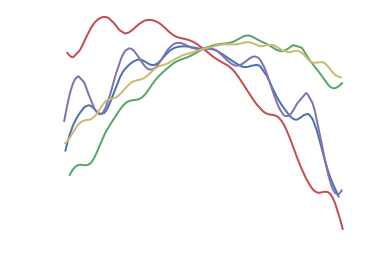
\includegraphics[width=.153\textwidth]{figs/gpSamples/main.png}
\begin{tikzpicture}


% level 1
\node (hyp) {\normalsize \color{blue} What is the probability of a trend, a recurring pattern {\bf and} noise in the data?};
\node[below = -0.2cm of hyp] (hyp_form) {$P\big((\text{LIN}\lor\text{LIN}\times\text{SE})\land
(\text{PER}\lor\text{PER}\times\text{SE}\lor\text{PER}\times\text{LIN})\land
(\text{WN}\lor\text{LIN}\times\text{WN})\big) = 0.36$};

%level 3
\node[below =.5cm of hyp_form , xshift=-3cm] (trend) {\color{blue} Is there a trend?};
\node[below = -0.2cm of trend] (trend_form) {$P(\text{LIN}\lor\text{LIN}\times\text{SE}) = 0.65$};
\node[below = -0.2cm of trend_form] (trend_png) {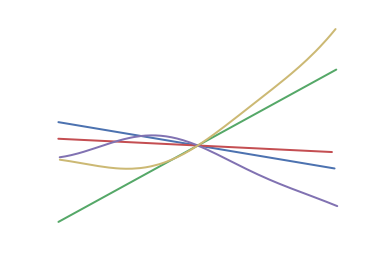
\includegraphics[width=.15\textwidth]{figs/gpSamples/trend.png}};

\node[below =.5cm of hyp_form, xshift=3cm] (noise) {\color{blue} Is there noise? };
\node[below = -0.2cm of noise] (noise_form) {$P(\text{WN}\lor\text{LIN}\times\text{WN}) = 0.75$};
\node[below = -0.2cm of noise_form] (noise_png) {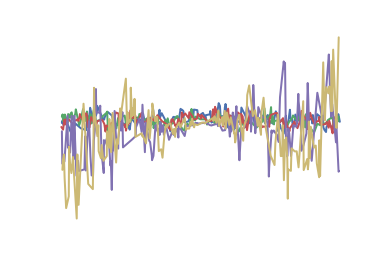
\includegraphics[width=.15\textwidth]{figs/gpSamples/noise.png}};

% level 4
\node[below =.5cm of trend_png , xshift=-2cm] (linear_trend) {\color{blue} A linear trend?};
\node[below = -0.2cm of linear_trend] (linear_trend_form) {$P(\text{LIN}) = 0.63$};
\node[below = -0.2cm of linear_trend_form] (linear_trend_png) {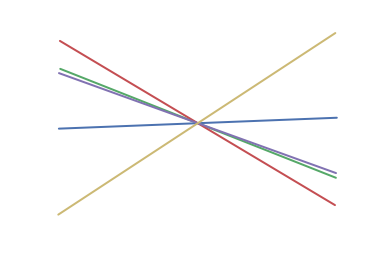
\includegraphics[width=.15\textwidth]{figs/gpSamples/lin.png}};

\node[below =.5cm of trend_png , xshift=1cm] (smooth_trend) {\color{blue} A smooth trend?};
\node[below = -0.2cm of smooth_trend] (smooth_trend_form) {$P(\text{LIN}\times\text{SE}) = 0.02$};
\node[below = -0.2cm of smooth_trend_form] (smooth_trend_png) {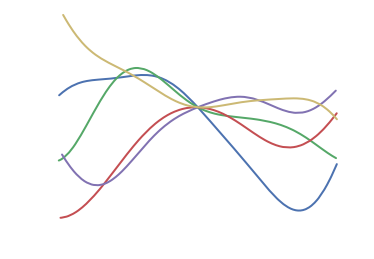
\includegraphics[width=.15\textwidth]{figs/gpSamples/selin.png}};

\node[below =.5cm of noise_png, xshift=-1cm] (het_noise) {\color{blue} Heteroskedastic noise? };
\node[below = -0.2cm of het_noise] (het_noise_form) {$P(\text{LIN}\times\text{WN}) = 0$};
\node[below = -0.2cm of het_noise_form] (het_noise_png) {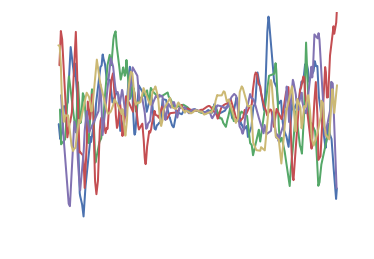
\includegraphics[width=.15\textwidth]{figs/gpSamples/linwn.png}};

\node[below =.5cm of noise_png, xshift=2cm] (white_noise) {\color{blue} White  noise? };
\node[below = -0.2cm of white_noise] (white_noise_form) {$P(\text{WN}) = 0.75$};
\node[below = -0.2cm of white_noise_form] (white_noise_png) {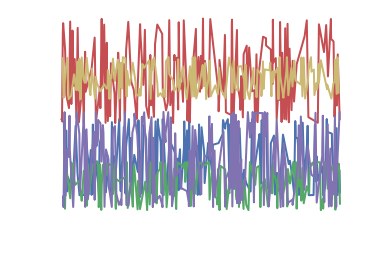
\includegraphics[width=.15\textwidth]{figs/gpSamples/wn.png}};

% level 5
\node[below =6.2cm of hyp_form] (recurring) {\color{blue} Is there repeating structure?};
\node[below = -0.2cm of recurring] (recurring_form) {$P(\text{PER}\lor\text{PER}\times\text{SE}\lor\text{PER}\times\text{LIN}) = 0.73$};
\node[below = -0.2cm of recurring_form] (recurring_png) {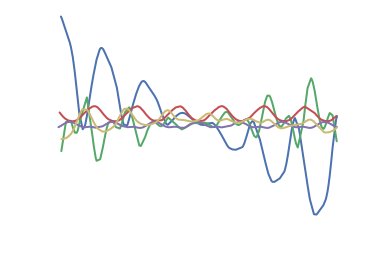
\includegraphics[width=.15\textwidth]{figs/gpSamples/recurring.png}};
%\draw[->,dashed] (barplot) -- (mcmc);

% level 6
\node[below =.5cm of recurring_png] (seper_form) {$\text{PER}\times\text{SE}=0.34$};
\node[below = -0.2cm of seper_form] (seper_png) {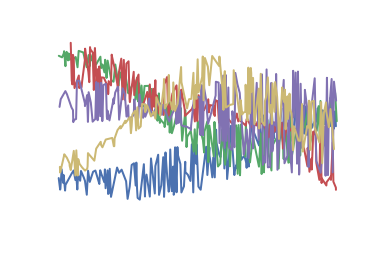
\includegraphics[width=.15\textwidth]{figs/gpSamples/seper.png}};

\node[below =.5cm of recurring_png, xshift=-3cm] (per_form) {$\text{PER}=0.32$};
\node[below = -0.2cm of per_form] (per_png) {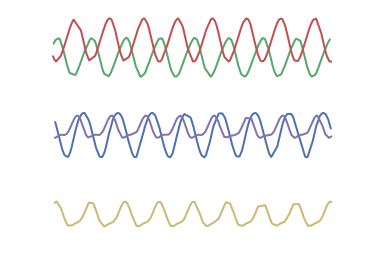
\includegraphics[width=.15\textwidth]{figs/gpSamples/per.png}};

\node[below =.5cm of recurring_png,xshift=3cm] (perlin_form) {$\text{PER}\times\text{LIN}=0.07$};
\node[below = -0.2cm of perlin_form] (seper_png) {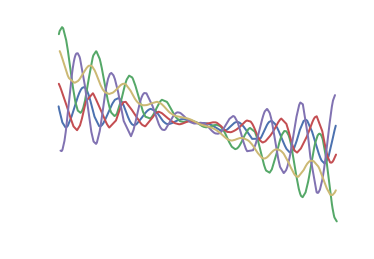
\includegraphics[width=.15\textwidth]{figs/gpSamples/perlin.png}};





\draw[->] (hyp_form) -- (trend);
\draw[->] (hyp_form) -- (noise);
\draw[->] (hyp_form) -- (recurring);


\draw[->] (noise_png) -- (het_noise);
\draw[->] (noise_png) -- (white_noise);

\draw[->] (trend_png) -- (linear_trend);
\draw[->] (trend_png) -- (smooth_trend);

\draw[->] (recurring_png) -- (per_form);
\draw[->] (recurring_png) -- (seper_form);
\draw[->] (recurring_png) -- (perlin_form);


\end{tikzpicture}



%  \multicolumn{3}{c}{$P(\text{PER}\lor\text{PER}\times\text{SE}\lor\text{PER}\times\text{LIN})$}

\caption{We can query the data if some logical statements are probable to be true, for example, is it true that there is a trend?}\label{fig:query}
\end{figure}